
\chapter{Automatic Viewpoint Selection for Interactive Motor Feedback Using Principle Component Analysis\label{sec:introduction}}
In our modern times, learning new skills is essential. May it be in recreational sports, physical therapy, or professions, skill learning is omnipresent. In addition, to improve the learning effect, skill learning can be supported by modern interactive technology. Particularly, in motor skill training supported by mixed reality technologies, interactive visual corrective feedback using motion tracking plays an increasingly important role as we showed in previous work~\cite{diller2022vcb}. Feedback is in this context used to teach people how to execute specific body movements correctly without the need for continuous supervision by highly qualified human trainers. Especially in physiotherapy and physical exercise, executing movements correctly is important to achieve the desired positive effects and avoid injuries. Furthermore, the context of physiotherapy and strength training involves controlled repetitive movements, which makes it possible to give clear feedback and identify typical mistakes. 

\begin{figure}[t!]
	\centering
	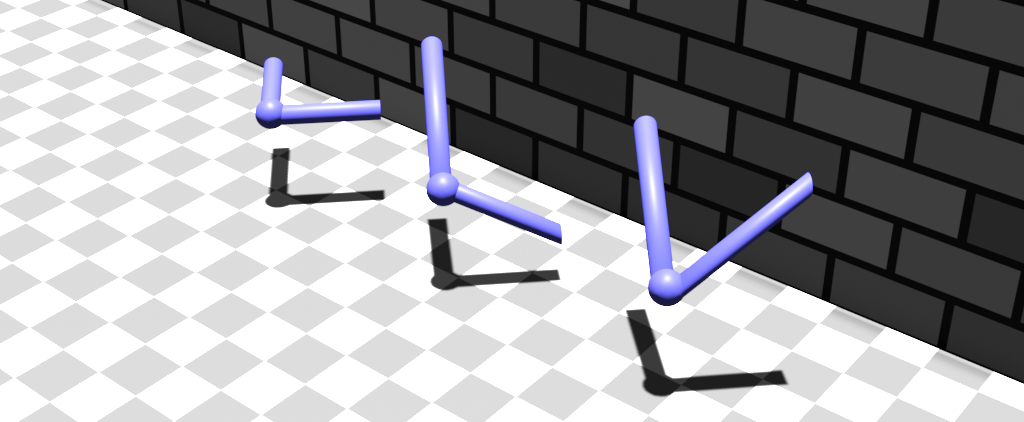
\includegraphics[width=\linewidth]{pictures/projection_normal.png}
	\caption{Example for the importance of viewpoint selection: Three \emph{different} angles at joints have the same shadow if projected to the ground. This implies they are also \emph{looking the same} when viewing them from above. Illustration inspired by Nundy et al.~\cite{nundy2000wam}.}
	\label{fig:projection_normal}
\end{figure}

\begin{figure*}[t!]
	\centering
	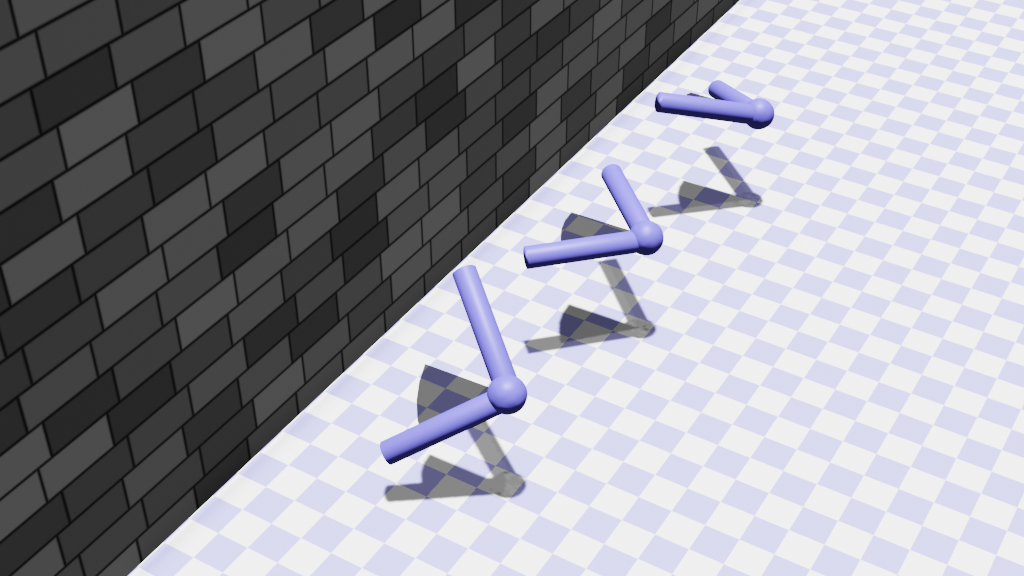
\includegraphics[width=0.49\linewidth]{pictures/projection_feedback}\hfill
	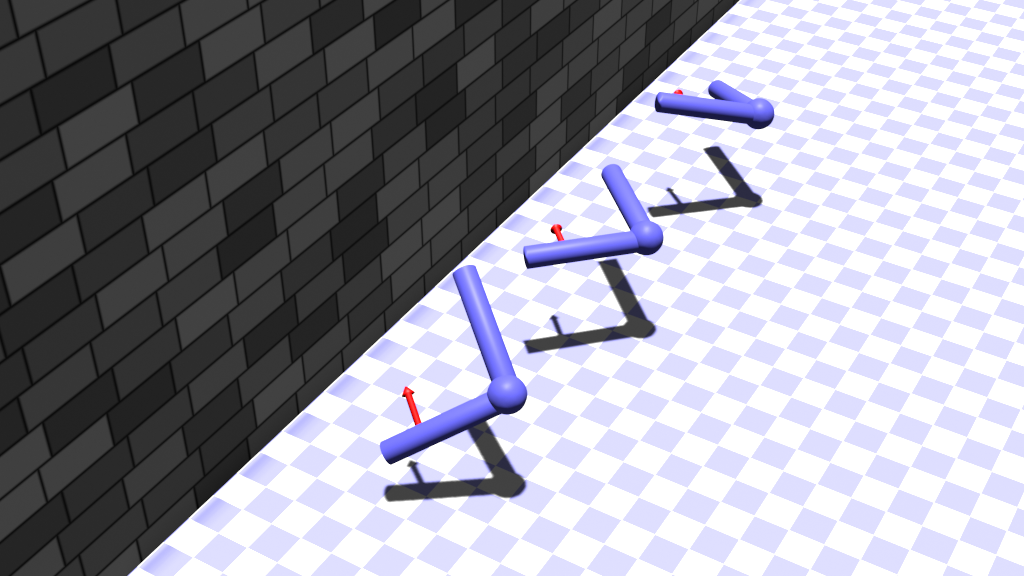
\includegraphics[width=0.49\linewidth]{pictures/projection_feedback_arrow}
	\caption{Feedback for the same angle viewed from different perspectives. Two different feedback cues: circular sector (left), and arrow (right). From left to right: Perfectly visible, visible, and hardly visible feedback. Shadows demonstrate that also for the feedback geometry, i.\,e.\,not only for the angle itself, but the viewpoint influences the perception.}
	\label{fig:projection_feedback}
\end{figure*}

If automatically generated feedback is rendered and displayed in real-time, a good viewpoint is crucial to allow users to correctly interpret, understand, and finally execute what is shown. Especially, the positions of the joints of the human skeleton and the angles between the respective limbs or bones are most relevant regarding the interpretation of executed movements. However, particularly for angles, the perception is highly dependent on the perspective. Previously analyzed by Nundy et al.~\cite{nundy2000wam}, angles are difficult for humans to perceive. That is especially true if rendered by a computer because a projection to the screen area is necessary and this projection can distort the angles as seen in \autoref{fig:projection_normal} and \autoref{fig:projection_feedback}. Regardless, while viewed in stereoscopy (e.g. real world or head-mounted displays), depth perception can help to interpret angles, and yet unfortunately that is not true to the same extent with a monoscopic rendering of an angle. However, the perception of angles is not the only obstacle faced when providing rendered feedback. Occlusion can also limit the understanding of the human pose in space. In particular, self-occlusion of the human avatar can hide limbs behind other body parts.
Likewise, if visual cues are rendered as feedback, they can be occluded by the avatar or by themselves as seen in figures~\ref{fig:projection_feedback} and~\ref{fig:skeletonFeedbackPerspective}. However, good visibility of the visual cues is central when giving corrective feedback. We recently showed the prevalent use of visual cues as corrective feedback for skill learning with mixed reality in the current literature~\cite{diller2022vcb}.

Nevertheless, feedback and visual cues in particular are not considered by current approaches for viewpoint selection regarding human motions and actions. Many methods found in the literature are computationally expensive and not real-time capable. In contrast, this paper gives insights into what factors are important when selecting viewpoints for movement correction and explains how these factors can be used to automatically select a viewpoint. Using \emph{principal component analysis} (PCA), we present a real-time capable algorithm to find a continuous optimal camera perspective for avatars of an actual motion together with a target motion and corresponding feedback. We validate the underlying assumptions and evaluate our methods in comparison to methods found in the literature in a user study. In addition, the results show that our method is not only preferred by users but also computationally the fastest.

\section{Related Work \label{sec:related}}	
As Bouwmans et al.~\cite{bouwmans2018arpca} showed for robust PCA, there are various uses for PCA in the field of visual computing. For example, Skaro et al.~\cite{skaro2021knac} present a method to reduce crosstalk errors, which are commonly present in marker-based motion tracking.

Several works discuss approaches of viewpoint selection for human actions or movements. For instance, Rudoy et al. \cite{rudoy2011vsh} create a volume from different frames to select the best physical camera for television broadcasts or similar applications. In contrast,  Kiciroglu et al. \cite{kiciroglu2020amc} provided an algorithm to predict the pose estimation accuracy to navigate a drone to the calculated position. Additionally, Shi et al. \cite{shi2012ksb} provide an algorithm to calculate the best viewpoint using the \emph{Kinematics Significance Based Saliency} to orient figures and objects preferring views that show most of the protruding features. 

Wang et al.~\cite{wang2019asw} achieve the selection of a single viewpoint of an action sequence utilizing information theory and deep reinforcement learning. Likewise, Choi et al.~\cite{choi2012rav} extract key frames from motion data to generate a sequence of stick figures to represent the initial motion data.

Ishara et al.~\cite{ishara2015mra} calculate the best camera position to navigate a robot with a camera mounted on top. For that purpose, the so-called \emph{Joint Mutual Occlusion} (JMO) is calculated by summating the angles between adjacent joints and the potential viewpoint. Concrete information like joint positions can be utilized, as the approach uses the information of a motion tracking camera. As a result, the work exhibits a close relation to our work, since we include motion-tracking data as well.

Similarly, Kwon et al. \cite{kwon2020ocp} use joint positions to calculate the best angle for skeletons utilizing projected limb lengths as well as 2D and 3D bounding boxes. Subsequently, the three metrics are combined in a weighted error function. Although these two approaches select camera positions for human poses automatically, they are not sufficient for visual feedback, as the skeleton can occlude the feedback. In addition, feedback provided can be difficult to perceive as analyzed by Nundy et al. \cite{nundy2000wam} and discussed in \autoref{sec:introduction}.

The last two approaches mentioned -\cite{ishara2015mra} and \cite{kwon2020ocp} - were compared to our method in the subsequent user study, as only these methods were possible to apply to human figures with feedback. For more information see \autoref{sec:relatedMethods}.

Another topic related to the viewpoint selection of an executed movement is camera path computation. For instance, Kwon and Lee~\cite{kwon2008dcp} describe how a smooth camera path can be computed using the area traversed by a movement when projected on the screen. Additionally, their method also considers occlusion.

Yeh et al.~\cite{yeh2011ecp} create smooth, aesthetic camera paths using a greedy-based tree traversal approach. In contrast, Assa et al.~\cite{assa2005asp} summarize actions using still images. Consequently, that requires the selection of key poses within the motion.

Assa et al.~\cite{assa2008moh} present a method to compute a camera path and give an overview of human actions. That involves among other indicators the third eigenvector generated by PCA of the joint coordinates as we do, as explained in \autoref{sec:methodology}. However, their use case varies drastically. As they are computing camera paths, it is acceptable to involve camera cuts. In contrast, we avoided this in our approach, as the exercise repetitions are short, so cuts in the camera movement are comparatively irritating to the viewers. Furthermore, the work of Assa et al. is action-based. Our work instead is feedback-based. That requires additional measures because our method must ensure the feedback is visible to the user. Lastly, their approach is not able to perform in real-time, as it is computationally expensive and requires the whole motion sequence for computation.

\begin{figure}[ht]
	\centering
	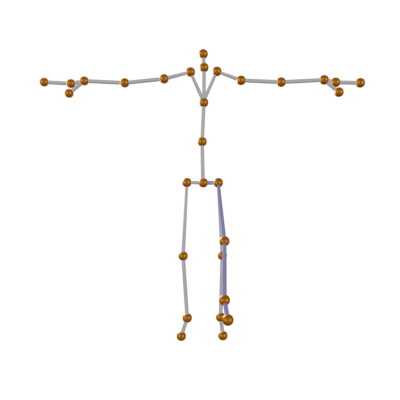
\includegraphics[width=0.49\linewidth]{pictures/skeleton_feedback_front}
	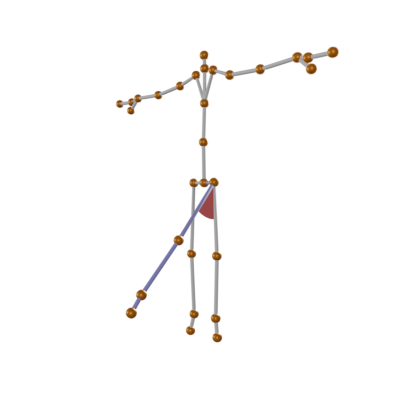
\includegraphics[width=0.49\linewidth]{pictures/skeleton_feedback_side}
	\caption{Skeleton of a human pose with feedback from two perspectives. Two visual feedback cues are shown: circular sector and additional avatar (here skeleton). The feedback is hardly visible from the perspective on the left.}
	\label{fig:skeletonFeedbackPerspective}
\end{figure}

\begin{figure}[ht]
	\centering    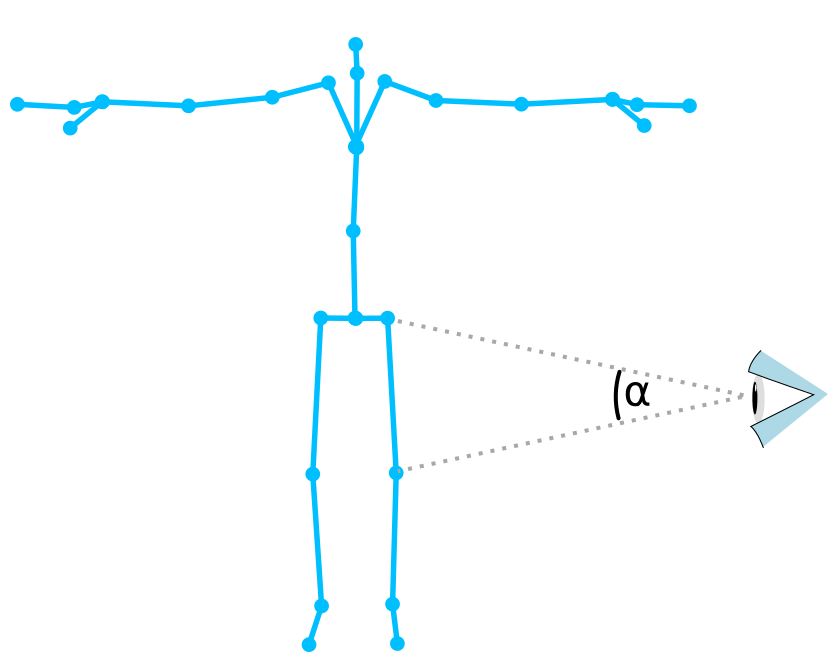
\includegraphics[width=\linewidth]{pictures/skeleton_E_occ.png}
	\caption{Measure for the self-occlusion of the skeleton by Ishara et al.~\cite{ishara2015mra}: Joint Mutual Occlusion.}
	\label{fig:jmo}
\end{figure}


\section{Perspective Considerations \label{sec:considerations}}
In the literature, we do not find absolute rules for good perspectives. However, we can extract several criteria and hints on what might be considered a good viewpoint. That includes both empirically established user preferences and logical argumentation.

\subsection{General Considerations}
Polonsky~et~al.~\cite{polonsky2005wii} identified seven measurable view descriptors. Yet they concluded, that finding a general way to provide a good view of an object is challenging. None of the seven view descriptors alone gives a general measure of viewpoint quality. However, there are some clues on how to treat certain objects. For example, Zusne~\cite{zusne1970vpf} empirically showed that if the object has eyes and a face, humans prefer to view it frontally.

As there is no general description of a good view, we need to define what characterizes a good viewpoint for our use case. In the following explanations, we often use the metaphor of a virtual camera, common in rendering to describe the viewpoint and viewing direction. Following Zusne's \cite{zusne1970vpf} findings, we prefer an approximately frontal view of the human pose, i.e. views where the virtual camera is pointed towards the front of the pose rather than a view from behind. Moreover, the camera up-vector should be the same as the world up-vector to avoid confusing the viewers since this is the biologically common way for humans to perceive. Additionally, we also want to limit the occlusions of the avatars showing the movement execution. Lastly, in our use case, we provide feedback through visual cues for correcting movement or poses and thus want this feedback to be visible. This means the feedback should not be occluded by the avatar or itself and should be as perpendicular to the view direction as possible.

When selecting perspectives for human motions and corresponding feedback, dependencies of different body parts are relevant. In particular, the limbs are hierarchically linked. Therefore, when we, for example, move the upper arm, the lower arm and hand will follow. Consequently, perspectives for such motions would ideally consider a \emph{hierarchical drill-down mechanism} to prioritize along the hierarchy.

\subsection{Methods from Current Literature \label{sec:relatedMethods}}
There are several methods to provide a good view of a human figure and limit self-occlusion as we described in \autoref{sec:related}. For instance, the JMO of Ishara et al.~\cite{ishara2015mra} considers the angle \(\alpha\) between two joints and the viewpoint, as seen in \autoref{fig:jmo}. Subsequently, the angles \(\alpha_{nm}\) between joints \(n\) and \(m\) are summed up and normalized, where \(n,m \in N\) and \(n \neq m\), and where \(N\) represents the number of joints. Combinatorically this creates \(\frac{N!}{2(N-2)!}\) calculations of \(\alpha\)~\cite{charalambides2002enumerative}.

The work of Kwon et al. \cite{kwon2020ocp} results in a weighted sum of the three metrics \emph{normalized limb length}, \emph{normalized area of a 2-D bounding box}, and \emph{normalized visible area of a 3-D bounding box}. However, this, in their case, best-performing algorithm is designed for still poses and requires calculation for each pose. As a consequence, in the case of videos, this would require a recalculation for each frame. Furthermore, they present an algorithm without recalculating the weights for each frame, which is the sum of the three metrics without weights.

PCA is often used to reduce dimensions in data sets for machine learning~\cite{sorzano2014sdr}. The principal components represent the independent main directions in which the data points spread. If we handle spatial data, three independent directions are involved. The first two principal components represent the main spread directions. Additionally, the third component offers a good view direction, or perspective, to observe the data points, because it is perpendicular to the first two. This is equivalent to a dimension reduction from three to two, as the rendered image of 3D objects only features two dimensions. Assa et al.~\cite{assa2008moh} use this method in their work to calculate camera paths (see \autoref{sec:related}). For more practical information on how we apply this see \autoref{sec:methodology}.

\section{Methodology \label{sec:methodology}}
The existing literature as presented in \autoref{sec:related} does not yet provide an optimal viewpoint calculation for human movement with visual feedback as it is suitable for skill learning. Most approaches are optimized for human actions. Consequently, feedback provided for the action could not be visible from the action-optimized viewpoint. In the following, we guide you through the steps of our computationally inexpensive way to calculate a viewpoint for human actions with feedback. \autoref{eq:viewpoint} shows the calculation of our view direction $\vec{v}_d$:

\begin{equation}
	\label{eq:viewpoint}
	\vec{v}_d = w \cdot \vec{v}_{S} + \sum_{n=1}^N (\Delta_n - \delta_0) \cdot \vec{v}_{Fn}
\end{equation}

To calculate $\vec{v}_d$ we require the following variables: \(w\) is a weight to balance out the impact of the view towards the whole skeleton and towards the feedback, the vector \(\vec{v}_S\) represents the viewpoint optimized for all joint coordinates (i.e. the actual skeleton), \(N\) is the number of joints exceeding a given deviation threshold \(\delta_0\), \(\Delta_n\) is the deviation of a joint to the intended target position, \(\delta_0\) is a constant deviation threshold, and lastly \(\vec{v}_{Fn}\) is the view direction optimized for the feedback, i.e. the deviating joint \(J_n\) and its corresponding joints as seen in \autoref{fig:eigenvector}. We do not consider rotations in particular, as they inevitably lead to a distance deviation as well.

Some motion capture systems present data as three-dimensional joint coordinates (see \autoref{sec:recording} for our data acquisition conditions). When we conduct a PCA over this point cloud of joint coordinates, the first two eigenvectors \(\vec{e}_{1S}\) and \(\vec{e}_{2S}\) represent the two main spatial dimensions the points spread out in. The third eigenvector \(\vec{e}_{3S} = \vec{v}_S\), which is perpendicular to the first two, then gives a good view direction $\vec{v}$ for all joints, as explained in \autoref{sec:relatedMethods}. Because the point cloud representing the whole skeleton is most spread out in the horizontal and vertical directions of the captured camera picture, the view direction \(\vec{v}_S\) is optimal for understanding and overall movements and poses. This method is also seen in Assa et al.~\cite{assa2008moh}.

As we want to focus on the feedback for the deviations of the exercises, we have to consider the deviating joints. For this purpose, we selectively apply viewpoint calculation. We conduct a PCA of the actual and the target joint coordinates and the corresponding parent joint coordinates as seen in \autoref{fig:eigenvector} for joints $J_n, n\in[1..N]$ exceeding a deviation threshold \(\delta_0\) of the distance between the actual to the target joint location. Consequently, the eigenvector \(\vec{e}_{3Fn}\) of the PCA is orthogonal to the plane optimally displaying joint \(J_n\), its parent, as well as the corresponding optimal joint position and its parent. This can be seen in \autoref{fig:eigenvector}, where the considered joint \(J_n\) is shown in red, the optimal joint position in orange, and the corresponding parent joints are depicted in blue.

This gives us the view direction \(\vec{e}_{3Fn} = \vec{v}_{Fn}\) for the feedback of joint $J_n$, where \(n\in[1..N]\) is an index out of the number $N$ of joints exceeding the deviation threshold \(\delta_0\) to their target counterparts. In \autoref{eq:viewpoint}, the multiplication  of $\vec{v}_{Fn}$ with \(\Delta_n\) (minus the threshold \(\delta_0\)) increases the impact of joints with higher deviations. This also naturally promotes a kind of hierarchical drill-down mechanism (see \autoref{sec:considerations}), since lower hierarchy joints usually have a higher absolute deviation, as they are impacted by the deviations of the higher hierarchy joints (intercept theorem). We subtract the threshold \(\delta_0\) to ensure a continuous camera movement so that the impact of deviating joints continuously increases (sets in) from zero. The sum of all $\vec{v}_{Fn}$ represents a feedback-optimized view direction for all joints exceeding the deviation threshold.

The skeleton-optimized view direction is weighted with the constant \(w\) to impact the balance between optimizing for the skeleton and feedback. Values of \(\delta_0 = 50\) and \(\ w = 3\delta_0 = 150\) yielded the best results in our experiments. This holds several implications:
\begin{itemize}
	\item The view directions (eigenvectors) resulting from the PCA are normalized. That means they have a length of 1. In the virtual 3D space we applied a scale of \(1\ unit = 1\ mm\). Consequently, the deviation threshold \(\delta_0\) is corresponding to \(50\ mm\).
	\item For the feedback view direction \(\vec{v}_{Fn}\)  of a single joint to have the same impact as the view direction for the entire skeleton ($\vec{v}_S$), the joint would need to have a deviation of 200 mm. This consists of a 50 mm minimal threshold plus 150 mm of the weight.
	\item The deviations of several joints together can exceed the threshold of 150 mm to have the same impact on the view as the skeleton as a whole.
	\item If multiple joints do not exceed the 50 mm minimal threshold the skeleton still has an impact of 100\% and the viewpoint is optimized for just the skeleton.
	\item Because we consider the absolute deviation (instead of relative to the parent), lower hierarchy joints are dependent on their parent joints. This creates a hierarchical drill-down mechanism as explained in \autoref{sec:relatedMethods}, where the joints closer to the torso have a higher impact.
\end{itemize}

To obtain the viewpoint for the virtual camera, we subtract the normalized view direction \(\vec{v}_d\) from the location of the focus point, which will be centered in the rendered frame (in our case the joint representing the pelvis location, since it is a central point of the body). With the multiplication of a constant, the distance to the focused point can be set. The digital equivalent of 2~m held the best results in our case, as all exercises were in frame at this distance. This, however, depends highly on the settings (e.g. focal length) of the virtual camera chosen for the intended application.

\begin{figure}[tb]
	\centering
	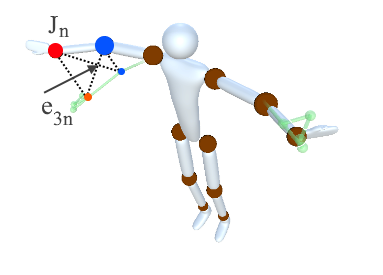
\includegraphics[width=\linewidth]{pictures/eigenvector.png}
	\caption{If Joint \(J_n\) (in red) deviates from the target position, we additionally include the corresponding target joint (in orange) and its parents (in blue) in the PCA. The eigenvector \(\vec{e}_{3n}\) then gives us an optimal view direction \(\vec{v}_{Fn}\) of the feedback. It is perpendicular to the plane defined by the eigenvectors \(\vec{e}_{1n}\) and \(\vec{e}_{2n}\). This plane does not interpolate the considered joints, but rather approximates their distribution.}
	\label{fig:eigenvector}
\end{figure}

If \(\vec{e}\) is an eigenvector, \(c \cdot \vec{e}\) is also an eigenvector, for all \(c \neq 0\)~\cite{borisenko}. Consequently, \(-\vec{v}_d\), the flipped eigenvector of \(\vec{v}_d\), is also viable as a view direction. Therefore we are free to choose which of the eigenvector orientations we use as our view direction. For the initial calibration, we can select the direction resulting in a more frontal view of the avatar, since this is the predominantly preferred view~\cite{zusne1970vpf}. For every further frame, we select the direction (out of the two) whose angular difference from the direction in the previous frame is smaller, as we want a smooth camera movement.

Although using the third eigenvector of the PCA results in a smooth camera movement, the camera tends to rotate around the avatar. Thus, the findings of Zusne~\cite{zusne1970vpf}, who stated humans prefer a frontal view, are contradicted. Hence, we projected view angles from behind to the frontal plane to solve this issue. This bypasses the predominantly small number of frames that feature a view from behind and shows a view from the side. The camera view is only slightly and very briefly affected by the projection.

Because the existing view selection approaches have foci different from ours, they rely on solving an optimization problem. As a consequence, often an algorithm iterates over a limited number of potential viewpoints, choosing the one with the best score. This either yields a costly high number of iterations or an erratic camera motion because the number of potential viewpoints is too small. Additionally, the best-scoring viewpoints in consecutive frames might be far from each other, which again results in inconsistent camera movements. However, our method provides a continuous camera movement, as the PCA computations are conducted for continuously moving point clouds, and none of the operations in \autoref{eq:viewpoint} compromises consistency.

In our exercise recordings, there were no cases where a null vector arose from our calculations. Additionally, we assessed stability regarding the PCA, as the camera view could flip if the second and third eigenvectors are approximately of the same length and deviate slightly. This was not the case in our experiments.

\section{Experimental Setup for Exercise Recording \label{sec:recording}}
The poses and motions used throughout this paper were recorded using a Microsoft Azure Kinect 3D camera~\cite{kinect:documentation}. Its computer vision capabilities deliver spatial coordinates of several joints of the human body it perceives. In the following, the term \emph{joint} is rather defined as biological points of interest than referring to the usual medical definition of joints~\cite{kinect:documentation}.

In the following, we describe the conditions that achieved optimal positioning of the subject in our case: The camera was elevated to a height of about 140~cm with the help of a tripod. It was placed at a distance of about 280~cm from the posing subject. The subject is about 190~cm tall. This gave us stable tracking and a clear frame for recording the poses. For our recordings, we discarded the joints of the eyes, ears, and nose as we found that these are too imprecise and they are irrelevant for pose correction in motor skill training. This left us with 26 joints. We compared two separate executions of the same exercise --- an ideal and current execution --- and showed corrective visual feedback cues to motivate the human user to decrease the difference and execute the motion correctly. For further information on the visualization of avatars see \autoref{sec:exercise}.

Subsequently, a set of example exercises was developed. This was done so various exercises and deviation combinations were included. We then compared each of these exercises to the corresponding counterpart with deviation from the correct form (see \autoref{sec:example}). The methods used to create a matching overlay of two exercises exceed the scope of this paper. We often see, for example, \emph{Dynamic Time Warping} fulfilling that role throughout literature~(e.g. \cite{su2013pre}, \cite{anton2015pre} and \cite{saenz2016kbv}).

\begin{figure}[b]
	\centering
	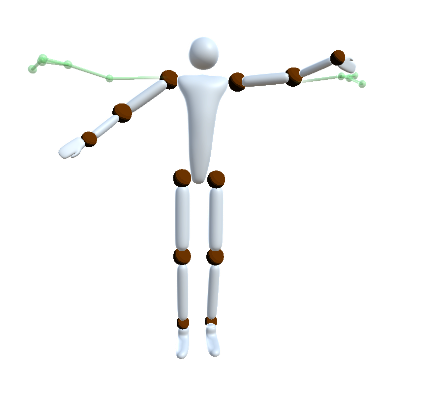
\includegraphics[width=\linewidth]{pictures/avatar.png}
	\caption{Example of the avatar and feedback used in the user studies. The white opaque avatar shows the actual movement, and the green transparent avatar shows the target movement.}
	\label{fig:avatar}
\end{figure}

\begin{figure*}[t!]
	\centering
	\subfloat[Bench press]{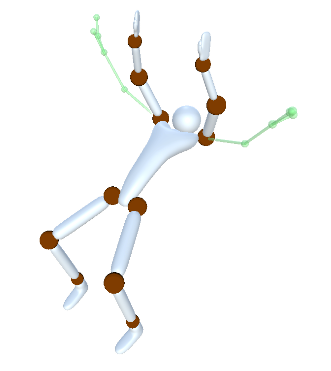
\includegraphics[width=.18\linewidth]{pictures/bench.png}\hfill}  
	\subfloat[Biceps curl A]{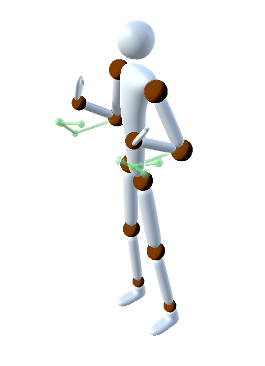
\includegraphics[width=.14\linewidth]{pictures/curlA.png}\hfill} 
	\subfloat[Lateral raises]{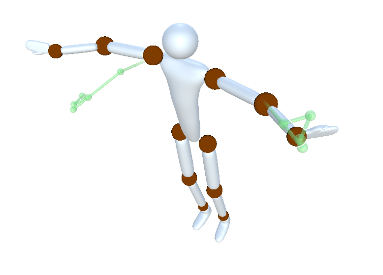
\includegraphics[width=.18\linewidth]{pictures/lateral.png}\hfill} 
	\subfloat[Shoulder press]{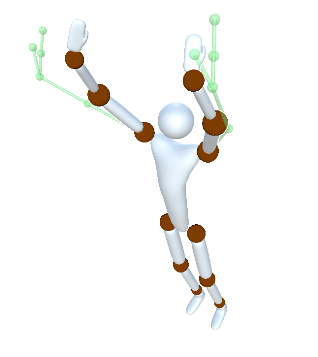
\includegraphics[width=.18\linewidth]{pictures/shoulder.png}\hfill} 
	\subfloat[Bend over row]{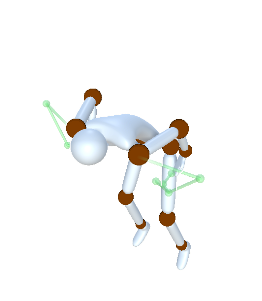
\includegraphics[width=.18\linewidth]{pictures/rows.png}\hfill}
	\subfloat[Biceps curl B]{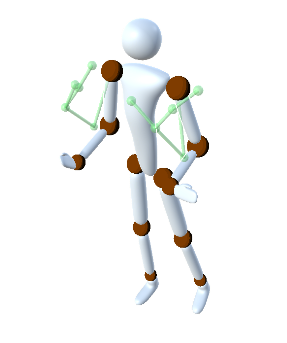
\includegraphics[width=.14\linewidth]{pictures/curlB.png}\hfill} 
	\caption{Example exercises with deviations as described in \autoref{sec:example}.}
	\label{fig:exercises}
\end{figure*}
\subsection{Exercise Visualization \label{sec:exercise}}
To visualize the actual motion we used an abstract avatar, and for the target motion, a skeleton is displayed as seen in \autoref{fig:avatar}. The visualization of the skeleton displayed in green corresponds to the joints recorded by the 3D camera~\cite{kinect:documentation} as mentioned in \autoref{sec:recording}. We used two different avatar visualizations to better distinguish the actual movement from the target movement. This also supports users with color vision deficiency, as the differences between the avatars are made clear by shape, not by color. The abstract avatar occludes more of itself and its background and visualizes fewer joint positions than the skeleton, as the fingertips and thumbs are integrated into the hand. Yet, for the optimization of the viewpoint, all joints are included in the calculations. The visualizations in this paper are just used for demonstrative purposes and are not the research subject. We focus on viewpoint selection, where the form of visualization plays a subordinate role.

\subsection{Example Exercises\label{sec:example}}

To evaluate our method (see~\autoref{sec:evaluation}) and compare it to approaches found in existing literature, we chose four still poses to establish basic assumptions and six moving exercises with corresponding deviations from the ideal form to evaluate different methods of viewpoint selection. The deviations were chosen to be typical mistakes for the exercises considered. We intended to find a selection of various exercises and deviations to evaluate the methods objectively. That means we selected the poses and exercises so that different movement and feedback directions are represented in the exercises. When performing lateral raises, for example, the arms are moved laterally away from the body, whereas, in a biceps curl, the arms move in front of the body (see \autoref{fig:exercises}). We also included an exercise with different deviations (biceps curls A and B).

Selecting a viewpoint for videos could be seen as selecting a continuous viewpoint for still poses in each frame. To confirm our underlying assumptions of viewpoint quality (see \autoref{sec:considerations}) we chose four representative still poses. In particular: Standing (standard anatomical position), squatting, bending down, and bench press.

In \autoref{sec:evaluation} we explain in detail how we let users select viewpoints and validate the results.

In the domain of physiotherapy and strength training many repetition-based exercises exist. We selected the following six exercises with deviations (see \autoref{fig:exercises} for visualization of the exercises): Bench press (Deviation: Arms too wide), Lateral raises (Deviation: Arms asymmetrical), Bend over row (Deviation: Elbows tucked in), Shoulder press (Deviation: Arms asymmetrical), Biceps curl A (Deviation: Repetition only half executed), and Biceps curl B (Deviation: Elbows do not stay stable).

%\begin{figure*}[t]
%    \centering
%    \subfloat[Bench press]{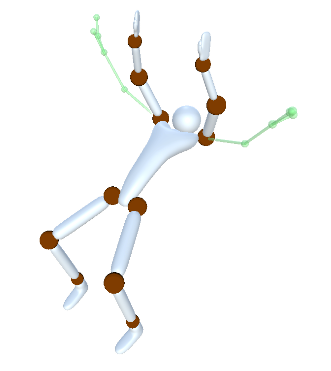
\includegraphics[width=.16\linewidth]{pictures/bench.png}}  
%    \subfloat[Biceps curl A]{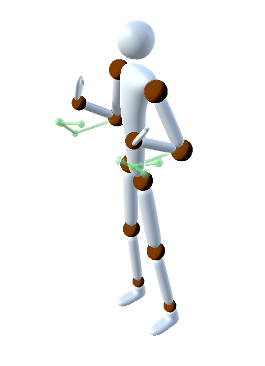
\includegraphics[width=.12\linewidth]{pictures/curlA.png}} 
%   \subfloat[Lateral raises]{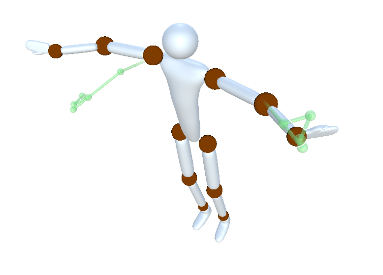
\includegraphics[width=.16\linewidth]{pictures/lateral.png}} 
%  \subfloat[Shoulder press]{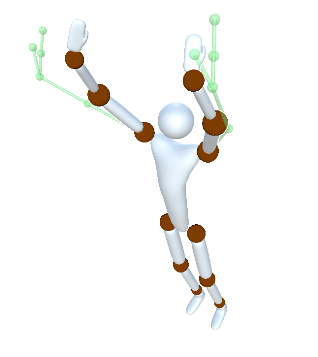
\includegraphics[width=.16\linewidth]{pictures/shoulder.png}} 
% \subfloat[Bend over row]{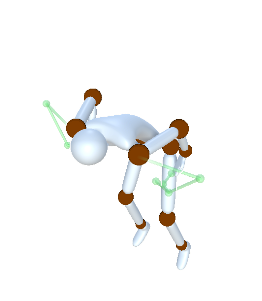
\includegraphics[width=.16\linewidth]{pictures/rows.png}}
%\subfloat[Biceps curl B]{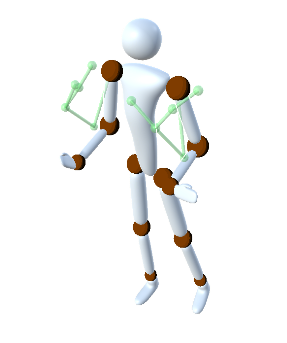
\includegraphics[width=.12\linewidth]{pictures/curlB.png}} 
%\caption{Example exercises with deviations as described in \autoref{sec:example}.}
%\label{fig:exercises}
%\end{figure*}


\section{Evaluation \label{sec:evaluation}}
For the evaluation of our method, we conducted a user study.
The user study was structured in three sections.

\textbf{Viewpoint Selection:} We intended to confirm our assumptions of user preferences for the views regarding our use case and compare it to the existing literature (primarily~\cite{zusne1970vpf}). For this purpose, we asked the users to choose the viewpoint for still poses. Feedback was not present in this section, as we wanted to evaluate the method for only the motions first. As a continuous camera movement for videos selects a viewpoint for a still pose in each frame, this should give us insights into what is preferred by the users and how our algorithm performs on that basic task without feedback. Furthermore, the selection of a camera path in real-time is unfeasible. Therefore, choosing still poses enables user evaluation. This makes it also possible to compare our method to the current literature (see \autoref{sec:related}).

A skeleton-like avatar successively showed four fixed poses of exercises: Bench press, squat, bend over row, and standing (for more information see \autoref{sec:example}). A skybox around the avatar helped with orientation in virtual 3D. The users were able to adjust the viewing angle for each pose by clicking and dragging the mouse. After confirmation, the viewpoint was registered.

\textbf{Viewpoint Comparison:} To evaluate the performance of our algorithm considering feedback, we showed a randomized juxtaposition of four looped videos of exercise repetitions with the corresponding correction feedback. The viewpoints in the four videos were each chosen by a different method. Six different exercises with deviations, as explained in \autoref{sec:example}, were successively shown.  

The different methods used for viewpoint selection included the \emph{JMO} of Ishara et al. \cite{ishara2015mra}, which chose the biggest sum of angles between all joints and the potential viewpoint. The method of Kwon et al.~\cite{kwon2020ocp} optimized the viewpoint of another exercise video. As their best resulting method is computationally intensive and not capable of real-time, we chose their algorithm variant without weights. For more information on the methods mentioned in this section see \autoref{sec:relatedMethods}. Our algorithm as described in \autoref{sec:methodology} was included as well. To compare the methods to a neutral position we included a viewpoint as it is used in isometric projection (rotated 45° horizontally, and 35.264° vertically).

\textbf{Questionnaire:} Finally, the third section allowed the participants to give more information about their previous engagement with the topic and asked for their opinions. The first four questions were asked using a Likert scale, the last two with free text:

\begin{itemize}
	\item How often do you exercise?
	\item How often are you involved in strength training?
	\item How often do you receive physiotherapy? 
	\item How often do you consider movements?
	\item What options you would have liked to see?
	\item What stood out to you?
\end{itemize}

\subsection{Participants \label{sec:participants}}
We acquired 39 individuals to participate in the user study. These were mainly computer science students between the ages of 20 and 30. Over half of the participants rated their frequency of exercise and motion-related considerations with four or higher out of five. This shows how well-acquainted the participants were with similar exercises and their execution. Physiotherapy clients were represented much less by comparison. Over half of the participants chose the lowest frequency of receiving physiotherapy. Color vision deficiency played no role in our user study. As we focused on perspective, only shapes needed to be recognized.

\subsection{Viewpoint Benchmark \label{sec:benchmark}}
We evaluated the registered viewpoints, chosen in the viewpoint selection section of the user study, using measures of the benchmark presented by Dutagaci et al.~\cite{dutagaci2010bbv}. They provided a method to evaluate a potential viewpoint and compare it to views chosen by users. \autoref{eq:vse} shows the calculation of what Dutagaci et al. call the \emph{View Selection Error} (VSE). The VSE is a number between 0 and 1, where low values represent a discrepancy to the chosen viewpoints.

\begin{equation}
	\label{eq:vse}
	VSE = \frac{1}{M \cdot \pi \cdot r}\sum_{m=1}^{M} GD_{m}
\end{equation}

\(GD_m\) represents the geodesic distances of the potential viewpoint to each chosen viewpoint \(m \in M\). $M$ stands for the number of participants (i.e. the number of viewpoints to consider). The distance of viewpoints to the object in focus is represented by \(r\). This could also be seen as the radius of a sphere on which all viewpoints lay (viewpoint sphere). To evaluate the viewpoints selected by the users, we projected the chosen viewpoint vectors on the median and transverse planes. Subsequently, we considered each degree a potential viewpoint around the focused object and plotted the \emph{View Selection Error} for each angle around the avatar representing the exercise in question. As a result, the \emph{View Selection Error} is displayed angle-wise in the median and frontal plane around the body using the Viridis colormap~\cite{viridis} in \autoref{fig:colorMaps}. Here, blue areas represent areas with a low view selection error and therefore a low distance to the view directions selected by the participants. In contrast, views that were avoided by the participants can be seen in yellow areas.


\begin{figure*}[ht]
	\centering
	\subfloat[Bench Press]{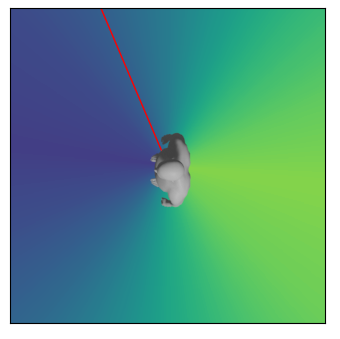
\includegraphics[width=0.24\linewidth]{pictures/transverseBench.png}}
	\subfloat[Squat]{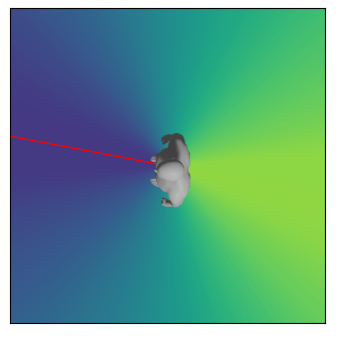
\includegraphics[width=0.24\linewidth]{pictures/transverseSquat.png}}
	\subfloat[Bend Down]{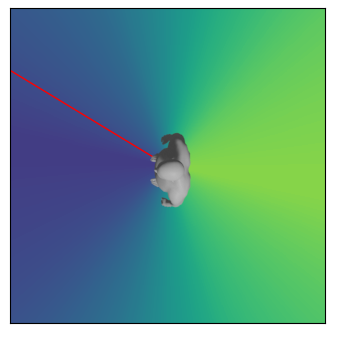
\includegraphics[width=0.24\linewidth]{pictures/transverseBend.png}}
	\subfloat[Stand]{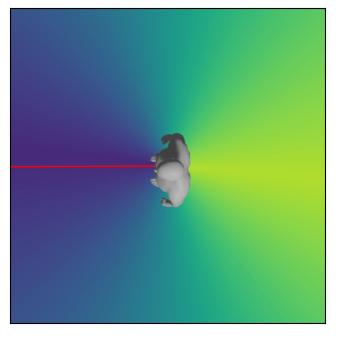
\includegraphics[width=0.24\linewidth]{pictures/transverseStand.png}}
\includegraphics[width=0.041\linewidth]{pictures/whitePixel.png}\\
	\subfloat[Bench Press]{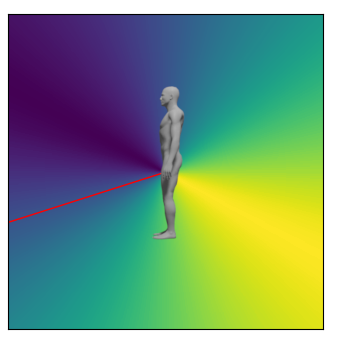
\includegraphics[width=0.24\linewidth]{pictures/medianBench.png}}
	\subfloat[Squat]{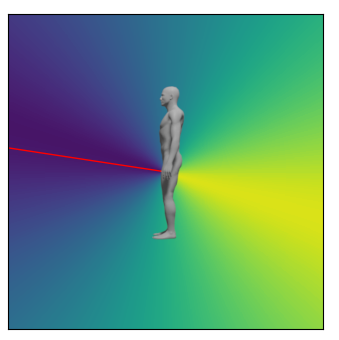
\includegraphics[width=0.24\linewidth]{pictures/medianSquat.png}}
	\subfloat[Bend Down]{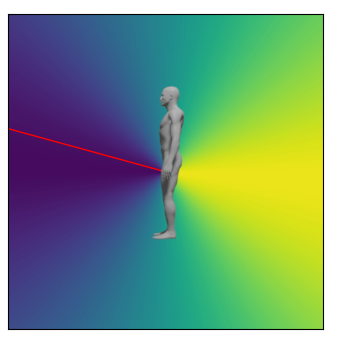
\includegraphics[width=0.24\linewidth]{pictures/medianBend.png}}
	\subfloat[Stand]{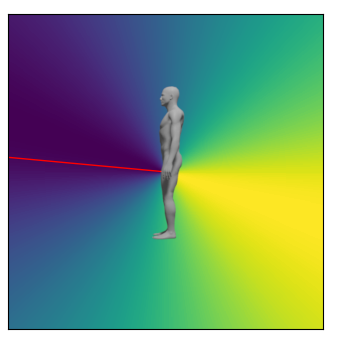
\includegraphics[width=0.24\linewidth]{pictures/medianStand.png}}    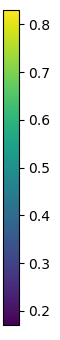
\includegraphics[width=0.041\linewidth]{pictures/scale.png}
	\caption{\emph{View Selection Error} (VSE) for different viewing angles from the top (a-d) and side (e-h) using the method of Dutagaci et al.~\cite{dutagaci2010bbv} without symmetry. The left represents the front. The red line represents the view direction selected by our method. The human silhouette is for spatial orientation only and does not represent the executed movements.}
	\label{fig:colorMaps}
\end{figure*}

\section{Results \label{results}}
In the following \autoref{sec:results:selection}, we will discuss how the basic viewpoint selection of each algorithm performed regarding the user-selected viewpoints utilizing the method explained in \autoref{sec:benchmark}. Subsequently, in \autoref{sec:results:analyis} we analyze how different algorithms compared displaying the same exercise by looking at the image sequences optimized by different methods. Lastly, \autoref{sec:results:comparison} concludes the results of the viewpoint comparison in the user study.

The results of the questionnaire are found in \autoref{sec:participants}, where they specify the participants, and in \autoref{sec:insights}, where the free-text answers are discussed.


\subsection{Viewpoint Selection \label{sec:results:selection}}
In \autoref{fig:colorMaps} blue areas represent a low view selection error. Therefore, viewpoints in these areas were close to the selection chosen by the participants of the user study. However, yellow areas were chosen less. Moreover, the red line represents the viewpoint our method chose for the still pose without movement.
The viewpoints calculated by our method predominantly match with the blue regions, i.e. in regions preferred by users. Likewise, when analyzing the view selection error mean over the four exercises, it becomes apparent that in comparison our algorithm fits the selection of the users best with a mean view selection error of 0.3467. The isometric-like view performed second best with 0.347 followed by JMO with 0.4825 and the method of Kwon et al. with 0.5497.

\subsection{Method Analysis\label{sec:results:analyis}}
To understand the comparison of methods in \autoref{sec:results:comparison}, it is crucial to comprehend what viewpoints the compared methods provide and how their succession appears over time.

\textbf{JMO~\cite{ishara2015mra}:}
The JMO algorithm employed predominantly a good overview of the human body. The biggest deficit was that the algorithm erratically changed viewpoints to positions far away from each other. This can be perceived in \autoref{fig:jmoSequence}. Consequently, the feedback was difficult to perceive, as the algorithm was not designed to display visual cues. Additionally, several viewpoints were selected from below, although participants preferred perspectives from slightly above (see \autoref{sec:results:selection}).

\textbf{Kwon et al.~\cite{kwon2020ocp}:} 
As \autoref{fig:kwonSequence} shows, the algorithm of Kwon et al. seemed to prefer views from behind in our examples. As elaborated in \autoref{sec:results:selection} this is an unusual view for humans and mostly avoided by users. In addition, views from below were occasionally selected like in the algorithm above. The algorithm of Kwon et al. provided a far more stable view than JMO. Although, the feedback was often difficult to see.

\textbf{Ours:}
Our algorithm provided a consistent transition between an optimal viewpoint for the neutral position to the contracted position with deviation as seen in \autoref{fig:bicepsSequence}. If feedback occurred it was displayed well and there was a perceivable emphasis on it. However, in some exercises the repetition execution was fast and the neutral and feedback-optimized viewpoints seemed conflicting. The result was a fast camera movement, which irritated some users.

\begin{figure*}[th]
	\centering
	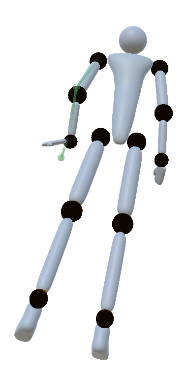
\includegraphics[width=0.11\linewidth]{pictures/jmoSequence1.png}\hfill
	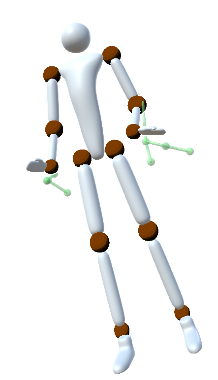
\includegraphics[width=0.12\linewidth]{pictures/jmoSequence2.png}\hfill
	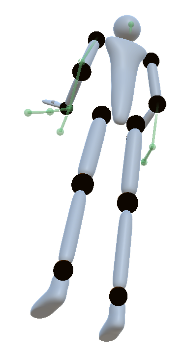
\includegraphics[width=0.12\linewidth]{pictures/jmoSequence3.png}\hfill
	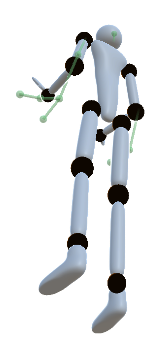
\includegraphics[width=0.10\linewidth]{pictures/jmoSequence4.png}\hfill
	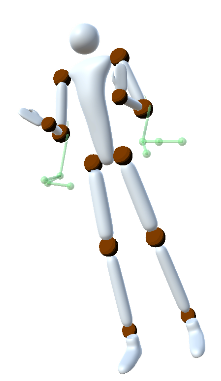
\includegraphics[width=0.12\linewidth]{pictures/jmoSequence5.png}\hfill
	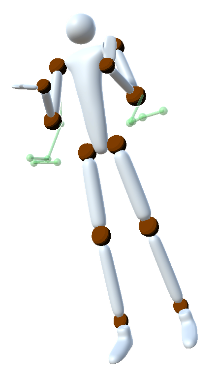
\includegraphics[width=0.12\linewidth]{pictures/jmoSequence6.png}\hfill
	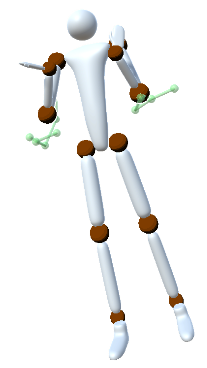
\includegraphics[width=0.12\linewidth]{pictures/jmoSequence7.png}\hfill
	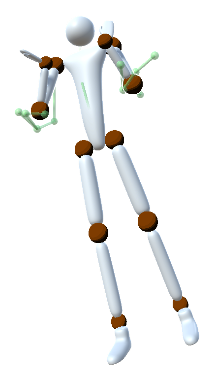
\includegraphics[width=0.12\linewidth]{pictures/jmoSequence8.png}\hfill
	\caption{Image sequence, taken from a video of a biceps curl exercise with deviation. The viewpoint is optimized by the \emph{Joint Mutual Occlusion} algorithm by Ishara et al.~\cite{ishara2015mra}.}
	\label{fig:jmoSequence}
\end{figure*}

\begin{figure*}[th!]
	\centering
	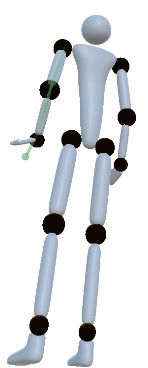
\includegraphics[width=0.11\linewidth]{pictures/kwonSequence1.png}\hfill
	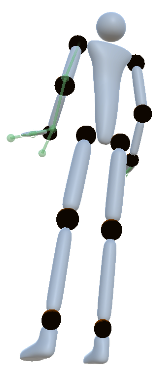
\includegraphics[width=0.12\linewidth]{pictures/kwonSequence2.png}\hfill
	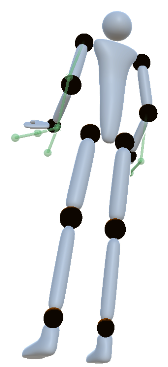
\includegraphics[width=0.12\linewidth]{pictures/kwonSequence3.png}\hfill
	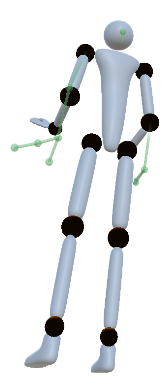
\includegraphics[width=0.12\linewidth]{pictures/kwonSequence4.png}\hfill
	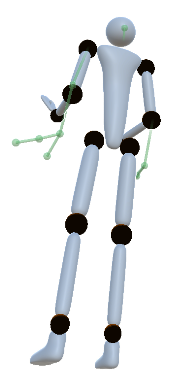
\includegraphics[width=0.12\linewidth]{pictures/kwonSequence5.png}\hfill
	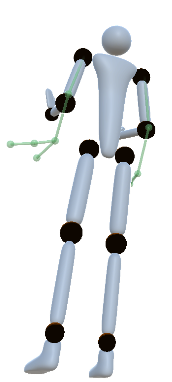
\includegraphics[width=0.12\linewidth]{pictures/kwonSequence6.png}\hfill
	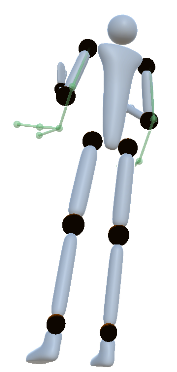
\includegraphics[width=0.12\linewidth]{pictures/kwonSequence7.png}\hfill
	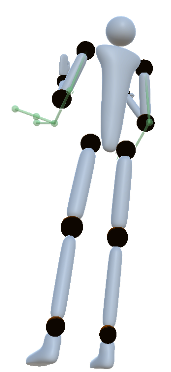
\includegraphics[width=0.115\linewidth]{pictures/kwonSequence8.png}\hfill
	\caption{Image sequence, taken from a video of a biceps curl exercise with deviation. The viewpoint is optimized by the algorithm by Kwon et al.~\cite{kwon2020ocp}.}
	\label{fig:kwonSequence}
\end{figure*}

\begin{figure*}[t!]
	\centering
	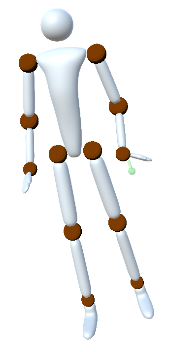
\includegraphics[width=0.115\linewidth]{pictures/bicepsSequence1.png}\hfill
	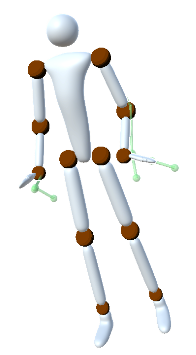
\includegraphics[width=0.13\linewidth]{pictures/bicepsSequence2.png}\hfill
	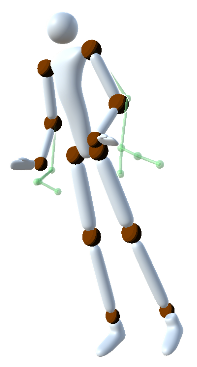
\includegraphics[width=0.125\linewidth]{pictures/bicepsSequence3.png}\hfill
	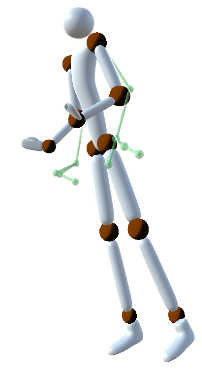
\includegraphics[width=0.125\linewidth]{pictures/bicepsSequence4.png}\hfill
	\includegraphics[width=0.12\linewidth]{pictures/bicepsSequence5.png}\hfill
	\includegraphics[width=0.115\linewidth]{pictures/bicepsSequence6.png}\hfill
	\includegraphics[width=0.11\linewidth]{pictures/bicepsSequence7.png}\hfill
	\includegraphics[width=0.11\linewidth]{pictures/bicepsSequence8.png}\hfill
	\caption{Image sequence, taken from a video of a biceps curl exercise with deviation. The viewpoint is optimized by our algorithm.}
	\label{fig:bicepsSequence}
\end{figure*}

\subsection{Viewpoint Comparison \label{sec:results:comparison}}
\autoref{tab:comparison} shows the distribution of user choices in the viewpoint comparison. Our algorithm was chosen most frequently with 35.04~\% of votes, the neutral position was chosen second most with 32.48~\% followed by Kwon et al.~\cite{kwon2020ocp} with 17.52~\% and lastly JMO~\cite{ishara2015mra} with 14.96~\%.

The methods of Kwon et al.~\cite{kwon2020ocp} and Ishara et al.~\cite{ishara2015mra} both occasionally provided camera positions from behind. Additionally, they produced a camera movement, which was unsteady because it jumped to perspectives and a limited number of viewpoints. In contrast, the static neutral viewpoint from the oblique front delivered surprisingly good results, although it lacked an adaption for movement or feedback. The biggest advantage of the neutral viewpoint compared to the other methods was the steadiness. Our method provided a good view of the neutral positions of the exercises. Furthermore, it produces a continuous camera movement toward a feedback-oriented viewpoint at the highest deviation. However, the camera movement showing the bench press and bend-over row exercises was in parts fast.

\begin{table}
	\begin{center}
		\resizebox{\columnwidth}{!}{
			\begin{tabular}{ |c|c|c|c|c|c|c|c| } 
				\hline
				\begin{sideways}Method\end{sideways} &\begin{sideways}Bench press\end{sideways} & \begin{sideways}Biceps curl A  \end{sideways} & \begin{sideways}Lateral raises\end{sideways} & \begin{sideways}Shoulder press\;\end{sideways} & \begin{sideways}Bend over row\end{sideways} & \begin{sideways}Biceps curl B\end{sideways} & \begin{sideways}\begin{tabular}{l}Total\\Percentage\end{tabular}\end{sideways} \\ 
				\hline\hline
				Neutral& 19 & 15 & 3 & 15 & 6 & 18 & 32.48~\% \\ 
				\hline
				JMO& 1 & 1 & 6 & 0 & 25 & 2 & 14.96~\% \\ 
				\hline
				Kwon & 14 & 7 & 3 & 3 & 6 & 8 & 17.52~\% \\ 
				\hline
				Ours & 5 & 16 & 27 & 21 & 2 & 11 & {\textbf{35.04~\%}} \\
				\hline
			\end{tabular}
		}
		\caption{\label{tab:comparison}Results of user study. Distribution of how often different viewpoint selection methods have been chosen by the participants.}
	\end{center}
\end{table}

\subsection{Computation Time}
Our algorithm performed the fastest compared to the other algorithms. JMO took an average of 200.83 ms for one frame to calculate. The algorithm presented in the work of Kwon et al. took 16.84 ms and ours 0.18 ms on average. The calculations were executed on an Intel(R) Core(TM) i7-8750H CPU with 2.21 GHz. The visualization and feedback generation needed additional ressources, which meant only our algorithm was able to run in real time for our application.

\section{Insights / Discussion \label{sec:insights}}
Looking at \autoref{fig:colorMaps} it becomes evident that a frontal view was highly preferred by the participants. This is consistent with the statement made by Zusne~\cite{zusne1970vpf}, that frontal views are desired by humans, as mentioned in \autoref{sec:considerations} and confirms these requirements for our use case. Furthermore, it can be observed that our participants preferred a view from slightly above.

In some of the exercises, our algorithm performs significantly less well. This can be attributed to the constantly smooth but occasionally fast camera movement. In particular, the bench press and bend-over row had fast-moving results regarding camera movement. As stated in \autoref{sec:methodology} our algorithm does not allow for inconsistent camera movement, yet fast camera motions can occasionally occur.

The most common statement made by the participants regarded the consistency of camera movement. Specifically, movements that were too fast or shaky were highly irritating to the users. This observation matches the research by Assa et al.~\cite{assa2008moh} analyzing camera paths. Furthermore, it was often stated that multiple camera perspectives would be beneficial for understanding the poses and feedback. This is especially interesting for future work and when applying suggested methods. In addition, some users wished for the option to choose no method, as they found none of the suggested perspectives fit. This implies that there are improvements to our algorithm, that need further assessment. Lastly, it was hard for some users to interpret poses without relation to the surroundings. This applied primarily to the bench press exercise, where a virtual bench representation might be helpful to interpret the lying posture of the avatar. Hence, it could be beneficial for the understanding to include surroundings when working with exercises including equipment like weights, benches, pull-up bars, etc. However, it must be remembered that additional rendered equipment could occlude the avatar or visual cues and make it more difficult to perceive the provided feedback.

\section{Conclusion}
The extent of \emph{interactive} support, that technology can provide when learning new skills, is steadily growing. Consequently, it becomes increasingly important to find fast and practical ways to implement functionalities at the foundation of human-computer interaction like viewpoint selection. We presented a novel method to consider real-time motion feedback in viewpoint selection at a computationally low cost. Furthermore, we describe a user study that showed that our algorithm was not only the fastest but also the one preferred by the users to display feedback. Considering the \emph{Nested Model for Visualization Design and Validation} of Munzner~\cite{munzner2009anm}, we outperformed the methods found in the current literature on the data/operation abstraction layer as well as the algorithm layer.

While we achieved satisfying results compared to methods found in the literature, there is still an opportunity for improvement. In particular, it became apparent that users disliked fast or inconsistent camera movements. This calls for an optimization that limits movement speed, while still optimally displaying feedback in real-time. As these appear to be conflicting goals, research into a solution representing a feasible compromise is needed.

The impact of a hierarchical drill-down mechanism for joints should be further researched. It might be interesting to link certain camera control aspects to the hierarchical dependency of joints, for example, zoom. This could potentially create a dynamic camera control, which makes it possible to display precisely the crucial corrections. However, to ensure this, it has to be further analyzed in which order humans correct their deviations optimally, what factors play into this, and how technology can support it.

When implementing motion feedback it could also help users understand the feedback to include several viewpoints and render props to help set the avatar in relation to its surroundings.

